\section{双机异步通信查询实现}
\subsection{原理分析}
S3C2440A 的通用异步收发器(UART)配有 3 个独立异步串行 I/O(SIO)端口,
每个都可以是基于中断或基于 DMA 模式的操作。即UART 可以通过产生中断或 DMA 
请求来进行 CPU 和 UART 之间的数据传输。\\
S3C2440A 的 UART 包括了可编程波特率,红外(IR)发送/接收,插入 1 个或 2 
个停止位,5 位、6 位、7 位或 8 位的数据宽度以及奇偶校验。\\
每个 UART 包含一个波特率发生器、发送器、接收器和一个控制单元,
波特率发生器可以由PCLK、FCLK/n 或 UEXTCLK(外部输入时钟)时钟驱动。\\
\\
原理图如下:\\
\begin{figure}[htbp]
  \centering
  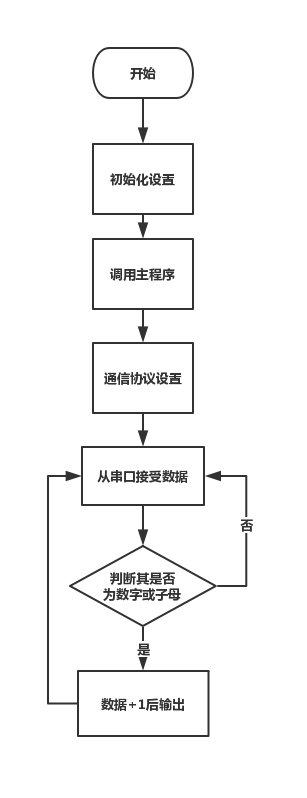
\includegraphics[width=0.3\textwidth]{sch2.png}
  \caption{双机异步通信查询实现原理图}
\end{figure}
\\
\\
\\

\subsection{调试过程}
\subsubsection{uart初始化程序}
head.s程序:\\
功能:初始化,设置clock和把代码搬到sdram快速运行。\\
\lstset{language=bash}
\begin{lstlisting}{初始化程序}
    bl  clock_init          @ 设置MPLL,改变FCLK、HCLK、PCLK
    bl  memsetup            @ 设置存储控制器以使用SDRAM
    bl  copy_steppingstone_to_sdram     @ 复制代码到SDRAM中
\end{lstlisting}
此段代码为初始化的核心,调用了各个初始化函数,如\lstinline{clock_init}。

\subsubsection{uart clock配置}
打开\lstinline{init.c},这里对clock进行配置,我们可以看到
\lstset{language=C}
\begin{lstlisting}{clock配置}
    #define S3C2410_MPLL_200MHZ     ((0x5c<<12)|(0x04<<4)|(0x00))
    #define S3C2440_MPLL_200MHZ     ((0x5c<<12)|(0x01<<4)|(0x02))
    void clock_init(void)
    {
        // LOCKTIME = 0x00ffffff;   // 使用默认值即可
        CLKDIVN  = 0x03;            // FCLK:HCLK:PCLK=1:2:4, HDIVN=1,PDIVN=1

        /* 如果HDIVN非0,CPU的总线模式应该从“fast bus mode”变为“asynchronous bus mode” */
        __asm__(
            "mrc    p15, 0, r1, c1, c0, 0\n"        /* 读出控制寄存器 */ 
            "orr    r1, r1, #0xc0000000\n"          /* 设置为“asynchronous bus mode” */
            "mcr    p15, 0, r1, c1, c0, 0\n"        /* 写入控制寄存器 */
            );

            /* 判断是S3C2410还是S3C2440 */
            if ((GSTATUS1 == 0x32410000) || (GSTATUS1 == 0x32410002))
            {
                MPLLCON = S3C2410_MPLL_200MHZ;  /* 现在,FCLK=200MHz,HCLK=100MHz,PCLK=50MHz */
            }
            else
            {
                MPLLCON = S3C2440_MPLL_200MHZ;  /* 现在,FCLK=200MHz,HCLK=100MHz,PCLK=50MHz */
            }       
    }
\end{lstlisting}
对于MPLLCON寄存器,[19:12]为MDIV,[9:4]为PDIV,[1:0]为SDIV
有如下计算公式:\\
\lstinline{MPLL(FCLK) = (2 * m * Fin)/(p * 2^s)}\\
其中: m = MDIV + 8, p = PDIV + 2, s = SDIV\\
对于本开发板,Fin = 12MHz,设置CLKDIVN,令分频比为:FCLK:HCLK:PCLK=1:2:4,\\
FCLK=200MHz,HCLK=100MHz,PCLK=50MHz

同时,打开\lstinline{interrupt.c},我们可以看到
\lstset{language=C}
\begin{lstlisting}{clock配置}
    ULCON0 &=0XFFFFFF00;
    ULCON0 |=0X03;      // 8N1(8个数据位,无较验,1个停止位)
    ///
    UCON0   = 0x05;     // 查询方式,UART时钟源为PCLK
    ///
    UFCON0  = 0x00;     // 不使用FIFO
    UMCON0  = 0x00;     // 不使用流控
    UBRDIV0 = UART_BRD; // 波特率为115200
\end{lstlisting}
这里把UART时钟源设置为PCLK,并且不使用FIFO,不使用流控,设置波特率为115200。\\
\\
S3C2440A 中的时钟控制逻辑可以产生必须的时钟信号,包括 CPU 的 FCLK,AHB 总线
外设的 HCLK 以及APB 总线外设的 PCLK。S3C2440A 包含两个锁相环(PLL):
一个提供给 FCLK、HCLK 和 PCLK,另一个专用于USB 模块(48MHz)。
时钟控制逻辑可以不使用 PLL 来减慢时钟,并且可以由软件连接或断开各外
设模块的时钟,以降低功耗。\\
\\
其中FCLK,HCLK 和 PCLK的分析如下:\\
FCLK 是提供给 ARM920T 的时钟。\\
HCLK 是提供给用于 ARM920T,存储器控制器,中断控制器,LCD 控制器,DMA 和 USB 主机模块的 AHB
总线的时钟。\\
PCLK 是提供给用于外设如 WDT,IIS,I2C,PWM 定时器,MMC/SD 接口,ADC,UART,GPIO,RTC 和
SPI 的 APB 总线的时钟。\\
S3C2440A 还支持对 FCLK、HCLK 和 PCLK 之间分频比例的选择。该比例由 CLKDIVN 控制寄存器中的 HDIVN
和 PDIVN 所决定。\\
分频比例如下:
\begin{figure}[htbp]
  \centering
  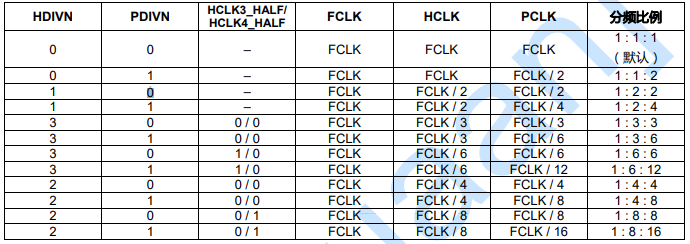
\includegraphics[width=0.8\textwidth]{uart1.png}
  \caption{分频比例}
\end{figure}

\subsubsection{uart循环发送程序}
我们为了能够直观看到结果,将main.c的代码修改成发送机子和接收机子。\\
\\
发送机子主程序:\\
功能:每次复位即向uart0发送a。\\
\lstset{language=bash}
\begin{lstlisting}{发送机子main.c程序}
    int main()
    {
        uart0_init(); 
        unsigned char c='a';
        putc(c);
        return 0;
    }
\end{lstlisting}
接收机子主程序:\\
功能:查询uart0。\\
\lstset{language=bash}
\begin{lstlisting}{接收机子main.c程序}
    int main()
    {
        unsigned char c;
        uart0_init(); 
        while(1)
        {
            c = getc();
            if (isDigit(c) || isLetter(c))
                putc(c+1);
        }
        return 0;
    }
\end{lstlisting}


\subsection{结果}
每次按下发送机子的复位键,接收机子即可接收到“a”。
\begin{figure}[htbp]
    \centering
    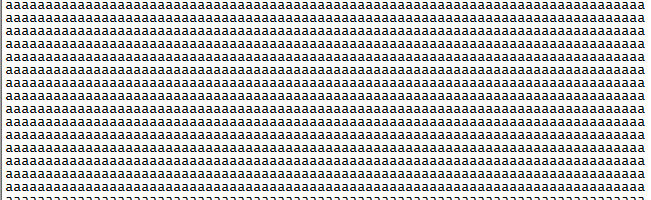
\includegraphics[width=0.8\textwidth]{result0.png}
    \caption{双机异步通信查询实现}
  \end{figure}
\subsection{问题与总结}
1. 原程序无法成功发送,需要自己看懂putc并发送。\\
2. 需要看原理图来查看哪一个管脚是发送,哪一个是接收。